\documentclass[convert]{standalone}

\usepackage{tikz}
\usepackage{graphicx}
\pagestyle{empty}

% INT_AY22_L11_Fig05_Vector_sum_diagram.png

\begin{document}
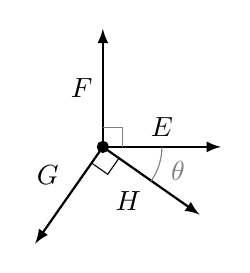
\begin{tikzpicture}[> = latex]

	% Define the ramp angle
	
	\def\Q{35}
	
	% The dot
	
	\filldraw (0, 0) circle (2 pt);
	
	% Four vectors
	
	\begin{scope}[->, thick]
	
		\draw (0, 0) -- node [above] {$E$} (0 : 1.5);
		\draw (0, 0) -- node [left] {$F$} (90 : 1.5);
		\draw (0, 0) -- node [above left] {$G$} (270 - \Q : 1.5);

		\draw (0, 0) -- node [below left] {$H$} (-\Q : 1.5);
		
	\end{scope}
	
	% Angle indicator for vectors E, H + perp squares
	
	\draw [gray] (0.75, 0) arc (0 : -\Q: 0.75);
	\node [gray] at ({-0.5 * \Q} : 1) {$\theta$};
	
	\draw [gray] (0.25, 0) -- (0.25, 0.25) -- (0, 0.25);
	
	\draw (-\Q : 0.25) -- ++ (270 - \Q : 0.25) -- ++ (180 - \Q : 0.25);
		
\end{tikzpicture}
\end{document}